\documentclass[]{elsarticle} %review=doublespace preprint=single 5p=2 column
%%% Begin My package additions %%%%%%%%%%%%%%%%%%%

\usepackage[hyphens]{url}

  \journal{Scientific Reports} % Sets Journal name

\usepackage{graphicx}
%%%%%%%%%%%%%%%% end my additions to header

\usepackage[T1]{fontenc}
\usepackage{lmodern}
\usepackage{amssymb,amsmath}
% TODO: Currently lineno needs to be loaded after amsmath because of conflict
% https://github.com/latex-lineno/lineno/issues/5
\usepackage{lineno} % add
\usepackage{ifxetex,ifluatex}
\usepackage{fixltx2e} % provides \textsubscript
% use upquote if available, for straight quotes in verbatim environments
\IfFileExists{upquote.sty}{\usepackage{upquote}}{}
\ifnum 0\ifxetex 1\fi\ifluatex 1\fi=0 % if pdftex
  \usepackage[utf8]{inputenc}
\else % if luatex or xelatex
  \usepackage{fontspec}
  \ifxetex
    \usepackage{xltxtra,xunicode}
  \fi
  \defaultfontfeatures{Mapping=tex-text,Scale=MatchLowercase}
  \newcommand{\euro}{€}
\fi
% use microtype if available
\IfFileExists{microtype.sty}{\usepackage{microtype}}{}
\usepackage[margin=3cm]{geometry}
\usepackage[]{natbib}
\bibliographystyle{plainnat}

\ifxetex
  \usepackage[setpagesize=false, % page size defined by xetex
              unicode=false, % unicode breaks when used with xetex
              xetex]{hyperref}
\else
  \usepackage[unicode=true]{hyperref}
\fi
\hypersetup{breaklinks=true,
            bookmarks=true,
            pdfauthor={},
            pdftitle={A rebuttal to Watters et al.~´2020 Long-term observations from Antarctica demonstrate that mismatched scales of fisheries management and predator-prey interaction lead to erroneous conclusions about precaution´},
            colorlinks=false,
            urlcolor=blue,
            linkcolor=magenta,
            pdfborder={0 0 0}}

\setcounter{secnumdepth}{0}
% Pandoc toggle for numbering sections (defaults to be off)
\setcounter{secnumdepth}{0}


% tightlist command for lists without linebreak
\providecommand{\tightlist}{%
  \setlength{\itemsep}{0pt}\setlength{\parskip}{0pt}}

% From pandoc table feature
\usepackage{longtable,booktabs,array}
\usepackage{calc} % for calculating minipage widths
% Correct order of tables after \paragraph or \subparagraph
\usepackage{etoolbox}
\makeatletter
\patchcmd\longtable{\par}{\if@noskipsec\mbox{}\fi\par}{}{}
\makeatother
% Allow footnotes in longtable head/foot
\IfFileExists{footnotehyper.sty}{\usepackage{footnotehyper}}{\usepackage{footnote}}
\makesavenoteenv{longtable}



\usepackage{booktabs}
\usepackage{longtable}
\usepackage{array}
\usepackage{multirow}
\usepackage{wrapfig}
\usepackage{float}
\floatplacement{figure}{H}
\newcommand{\pandocbounded}[1]{#1}
\usepackage{colortbl}
\usepackage{pdflscape}
\usepackage{tabu}
\usepackage{threeparttable}
\usepackage{threeparttablex}
\usepackage[normalem]{ulem}
\usepackage{makecell}
\usepackage{xcolor}
\usepackage{booktabs}
\newcommand{\blandscape}{\begin{landscape}}
\newcommand{\elandscape}{\end{landscape}}
\usepackage{float} \floatplacement{figure}{H}
\newcommand{\beginsupplement}{\setcounter{table}{0}
\renewcommand{\thetable}{S\arabic{table}}     -   - \setcounter{figure}{0}
\renewcommand{\thefigure}{S\arabic{figure}}}
\usepackage{booktabs}
\usepackage{longtable}
\usepackage{array}
\usepackage{multirow}
\usepackage{wrapfig}
\usepackage{float}
\usepackage{colortbl}
\usepackage{pdflscape}
\usepackage{tabu}
\usepackage{threeparttable}
\usepackage{threeparttablex}
\usepackage[normalem]{ulem}
\usepackage{makecell}
\usepackage{xcolor}



\begin{document}


\begin{frontmatter}

  \title{A rebuttal to Watters et al.~´2020 Long-term observations from
Antarctica demonstrate that mismatched scales of fisheries management
and predator-prey interaction lead to erroneous conclusions about
precaution´}
    \author[1]{Andrew Lowther%
  %
  }
  
    \author[2]{Ulf Lindstrøm%
  %
  }
  
    \author[3]{Bjørn Krafft%
  %
  }
  
    \author[4]{Javier A. Arata%
  %
  }
  
      \cortext[cor1]{Corresponding author}
  
  \begin{abstract}
  
  \end{abstract}
  
 \end{frontmatter}

\hypertarget{tables}{%
\section{Tables:}\label{tables}}

Table 1. Estimates of the mean (mu) and standard deviation (sd) of
Ln(LKB) by gSSMU and SAM sign, derived from Equation (2) of Watters et
al.~(2020). Statistical results from the nonparametric one-way ANOVA are
reported as follows: p-value\_1 compares SAM sign within each gSSMU, and
p-value\_2 compares gSSMUs within each SAM sign. The corresponding LKB
estimates appear in the column labelled mean LKB.

\begin{longtable}[]{@{}rlrrrrrr@{}}
\toprule\noalign{}
gSSMU & sam.sign & n & mu & sd & p-value\_1 & Median\_LKB &
p-value\_2 \\
\midrule\noalign{}
\endhead
\bottomrule\noalign{}
\endlastfoot
1 & Neg & 6 & 13.643 & 1.315 & 0.262 & 841401.3 & 0.071 \\
1 & Pos & 10 & 14.315 & 0.994 & NA & 1647467.9 & NA \\
2 & Neg & 6 & 14.809 & 0.681 & 0.096 & 2701181.9 & NA \\
2 & Pos & 10 & 15.512 & 0.792 & NA & 5456188.0 & 0.007 \\
\end{longtable}

\newpage

\hypertarget{figures}{%
\section{Figures:}\label{figures}}

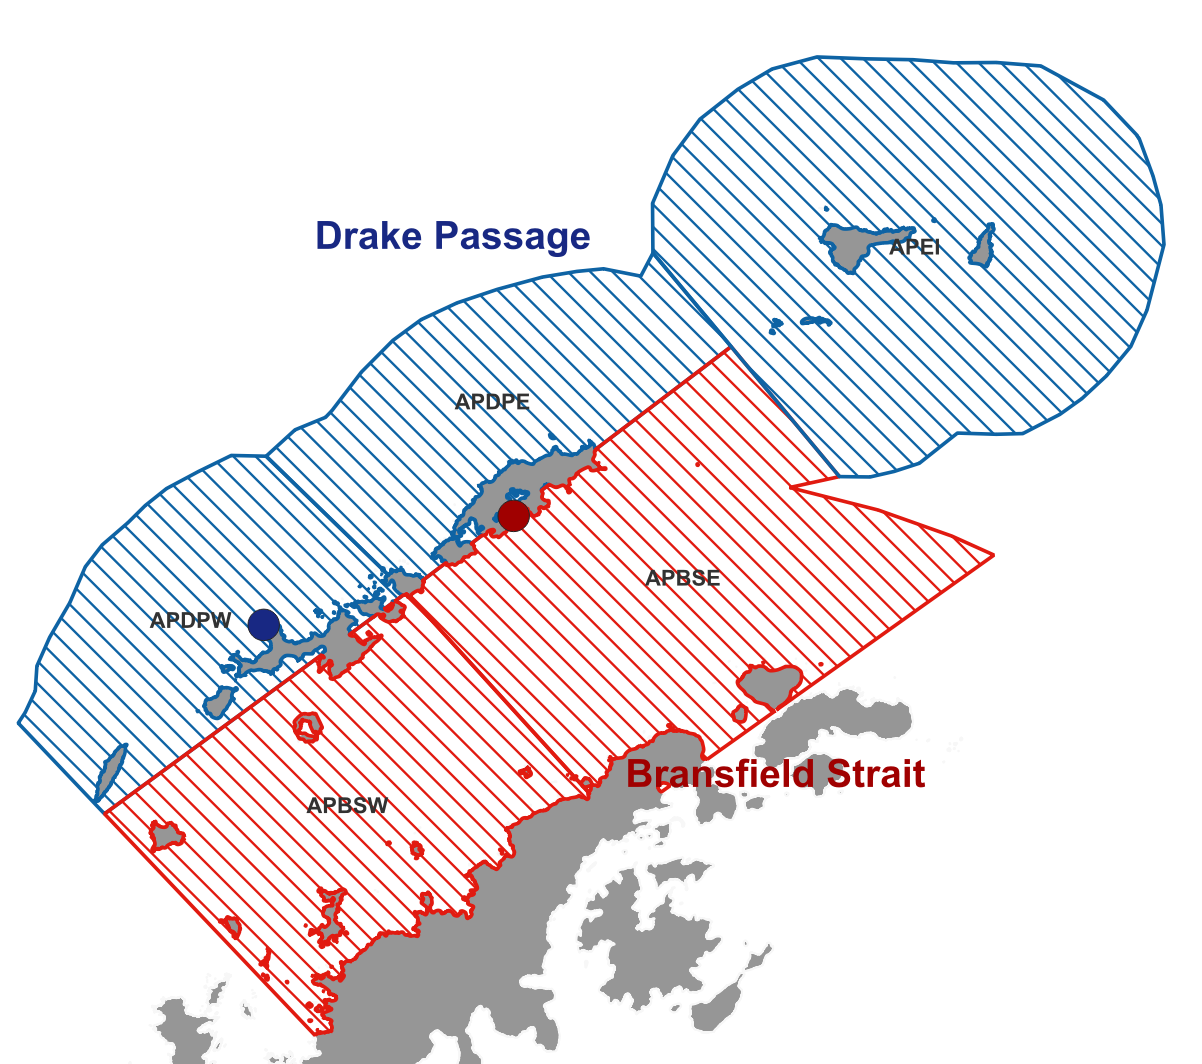
\includegraphics[width=1\linewidth]{./A_Results/Fig1_gSSMUs}

Figure 1. Locations of the penguin colonies (COPA shown in red, SHIRREF
shown in blue), the two gSSMUs (gSSMU 1 in the blue dashed area and
gSSMU 2 in the red dashed area), and the surrounding SSMUs (APEI:
Antarctic Peninsula Elephant Island; APDPE: Antarctic Peninsula Drake
Passage East; APDPW: Antarctic Peninsula Drake Passage West; APBSE:
Antarctic Peninsula Bransfield Strait East; APBSW: Antarctic Peninsula
Bransfield Strait West).

\includegraphics[width=0.8\linewidth]{WattKrug_Results_files/figure-latex/LKB vs SAM-1}
\includegraphics[width=0.8\linewidth]{WattKrug_Results_files/figure-latex/LKB vs SAM-2}

Figure 2. (A) Observed and imputed LKB (local krill biomass) by gSSMU
and summer SAM value. The dashed black line marks 1 Mt. Red and blue
dashed lines show mean values during negative SAM summers, and red and
blue solid lines show mean values during positive SAM summers (see Table
1). (B) Boxplots of observed LKB by gSSMU and SAM sign. Black, blue and
red lines as in figure (A). gSSMU 1 is shown in red and gSSMU 2 in blue.

\begin{landscape}

\includegraphics[width=1\linewidth]{WattKrug_Results_files/figure-latex/LKB vs LHR-1}

Figure 3. Krill survey estimates (LKB) for the study period. Top panel:
gSSMU 2 (SSIW-EI). Bottom panel: gSSMU 1 (BS). Filled circles show
survey data from Watters et al.~2020. Open circles show the mean imputed
median LKB values for negative and positive SAM, as per Table 1. Color
code: red = summer; blue = winter.

\end{landscape}
\begin{figure}
\includegraphics[width=0.65\linewidth]{./Watters EMM figures/Penguin distributions} \caption{Penguin foraging behaviour during summer breeding, derived from available ARGOS-CLS PTT data presented in Hinke et al. 2017. A) Chinstrap penguins from Cape Shireff (blue) and Copacabana (green) truncated at $10^{th}$ March in line with known phenology (Black 2016; Lowther et al.(this meeting).  Elongated grey track represents a single animal) B) Adélie penguins truncated to the end of January and C) gentoo penguins until \textasciitilde{}August, representing all available PTT data provided. The SSMU are combined and coloured according to gSSMU (red; gSSMU 2, purple; gSSMU 1) with chinstrap and Adélie penguin 99\% MCP home ranges occupying between 7-19\% of the gSSMU to which they were assigned.}\label{fig:Penguin distribution plots}
\end{figure}

\begin{figure}
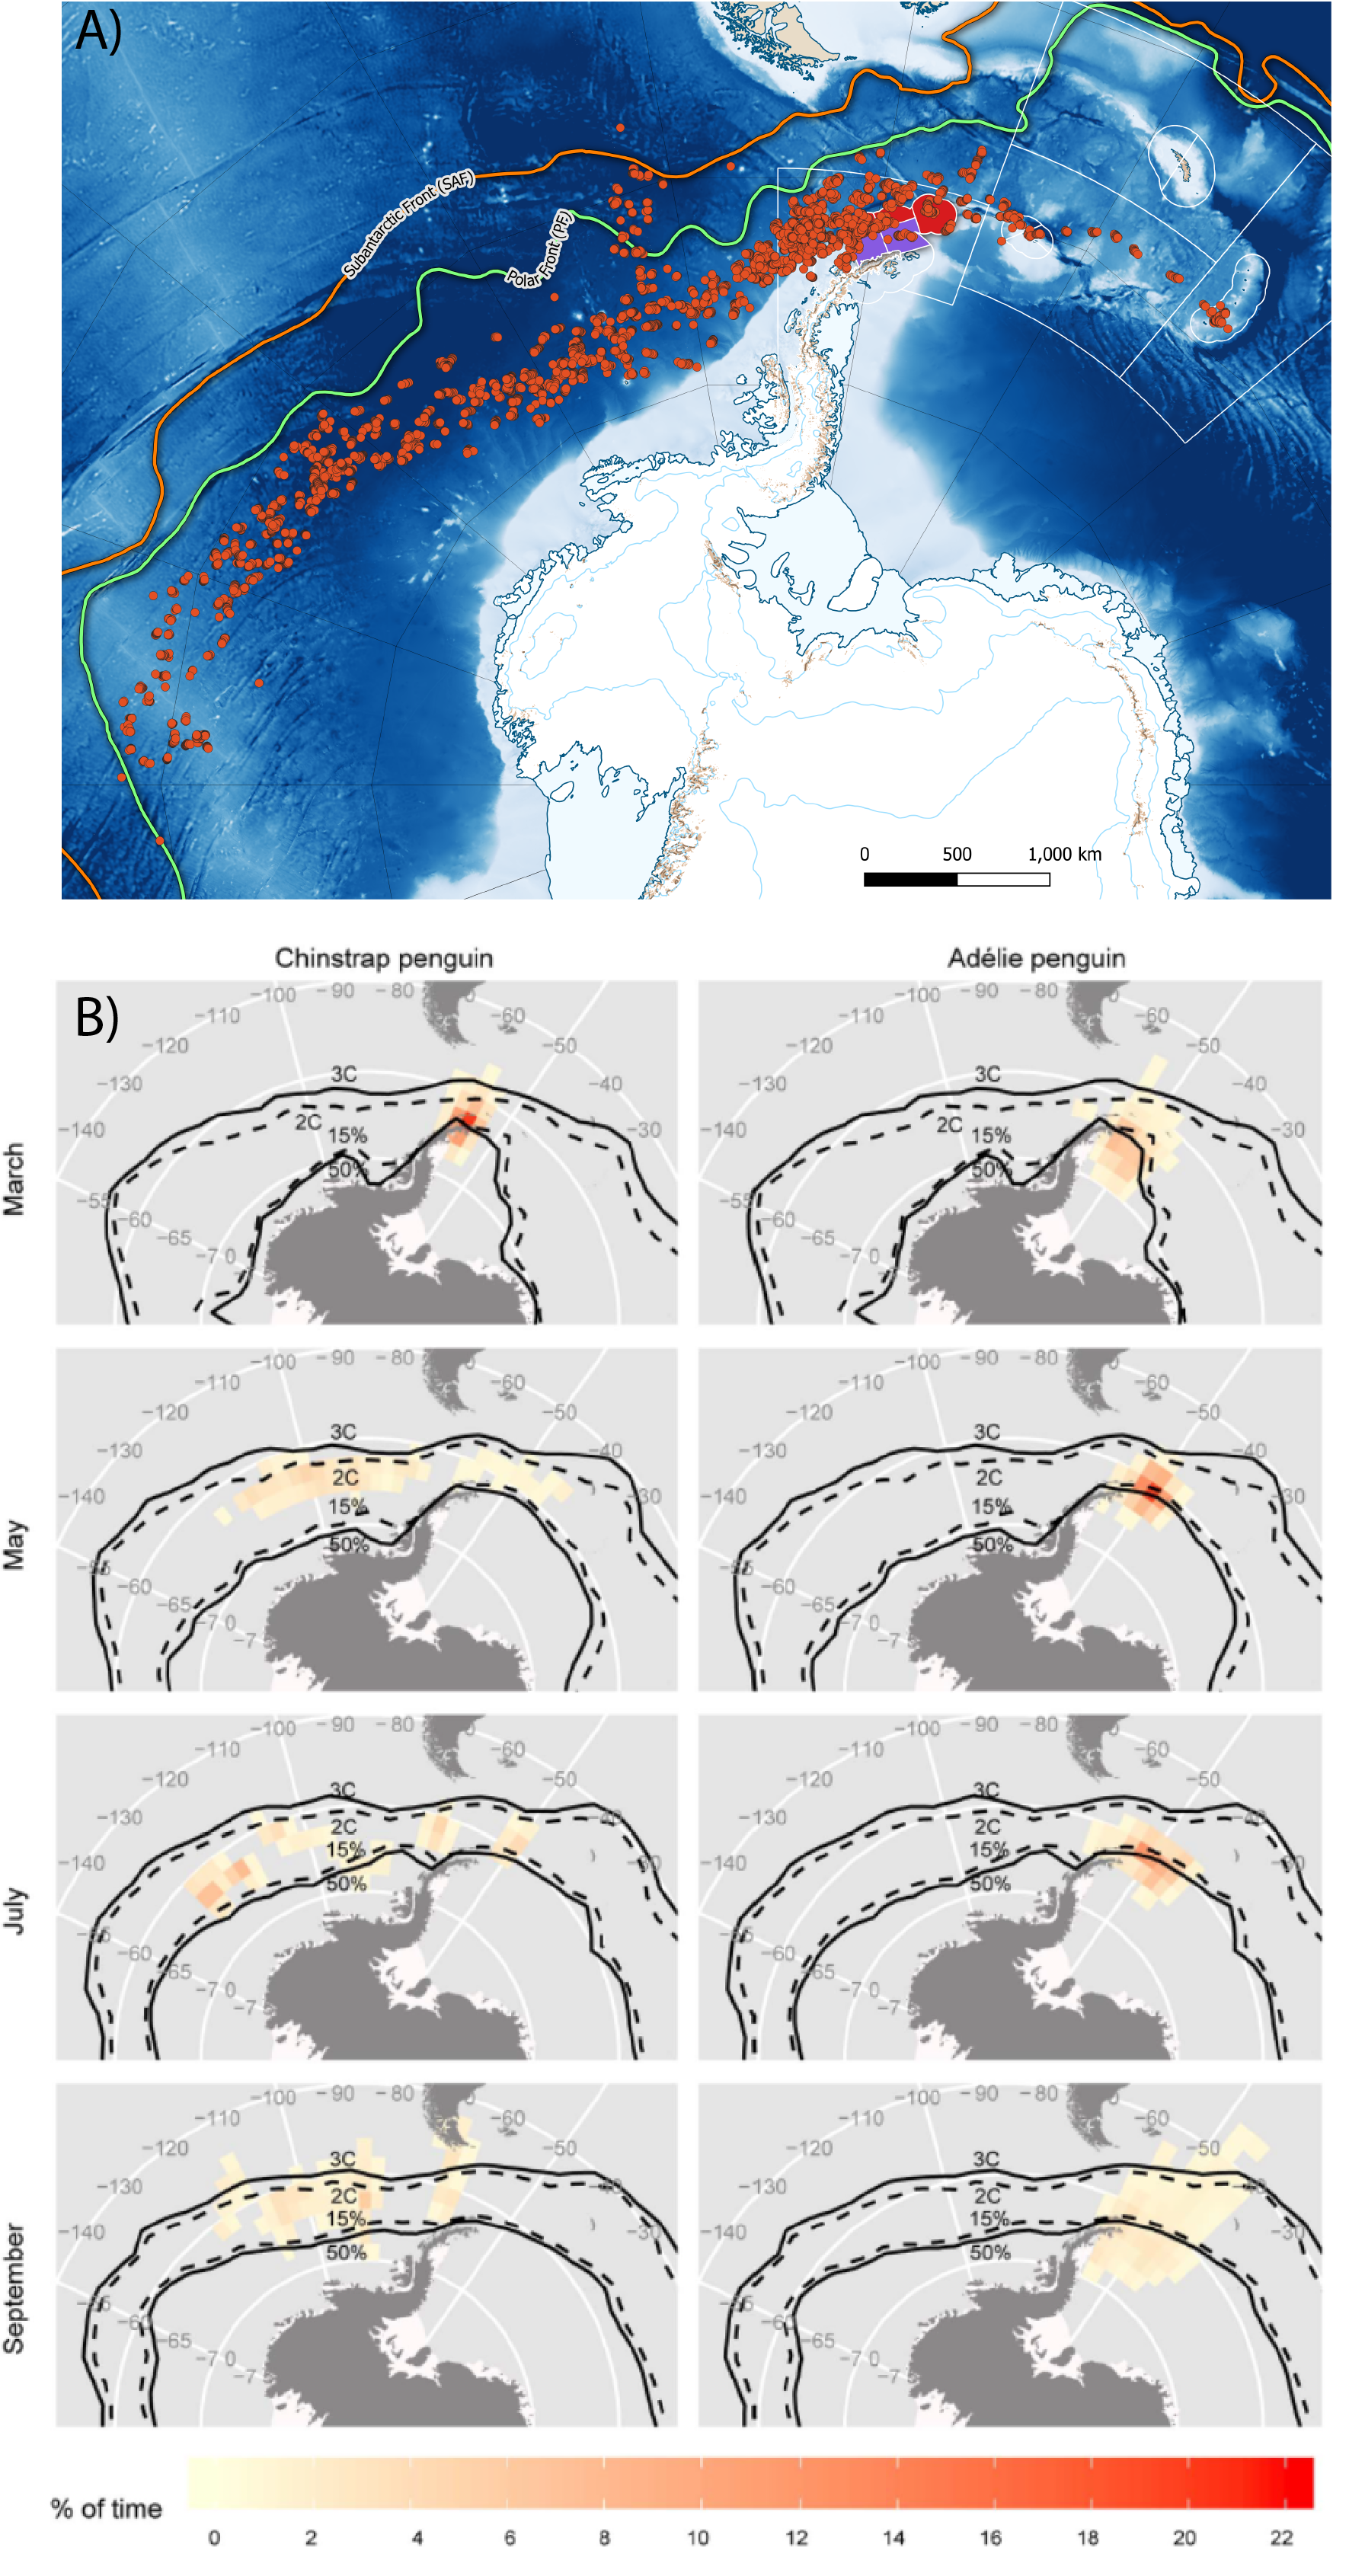
\includegraphics[width=0.75\linewidth]{./Watters EMM figures/Overwinter pengo distributions} \caption{A) Distribution of overwinter movement for chinstrap penguins, relative to the gSSMU's to which they were attributed, created from telemetry data available in Hinke et al. 2019.  B) Adélie and chinstrap penguin movement recorded by light geolocators, highlighting the large longitudinal range both species disperse through at the end of breeding (taken from Hinke et al. 2015).  In the original model formulation by Watters et al. 2020, the winter performance indices for both species are matched to macroscale levels of ONI variability but gSSMU-scale estimates of LKB and LHR.}\label{fig:Overwinter penguin  plots}
\end{figure}

\begin{figure}
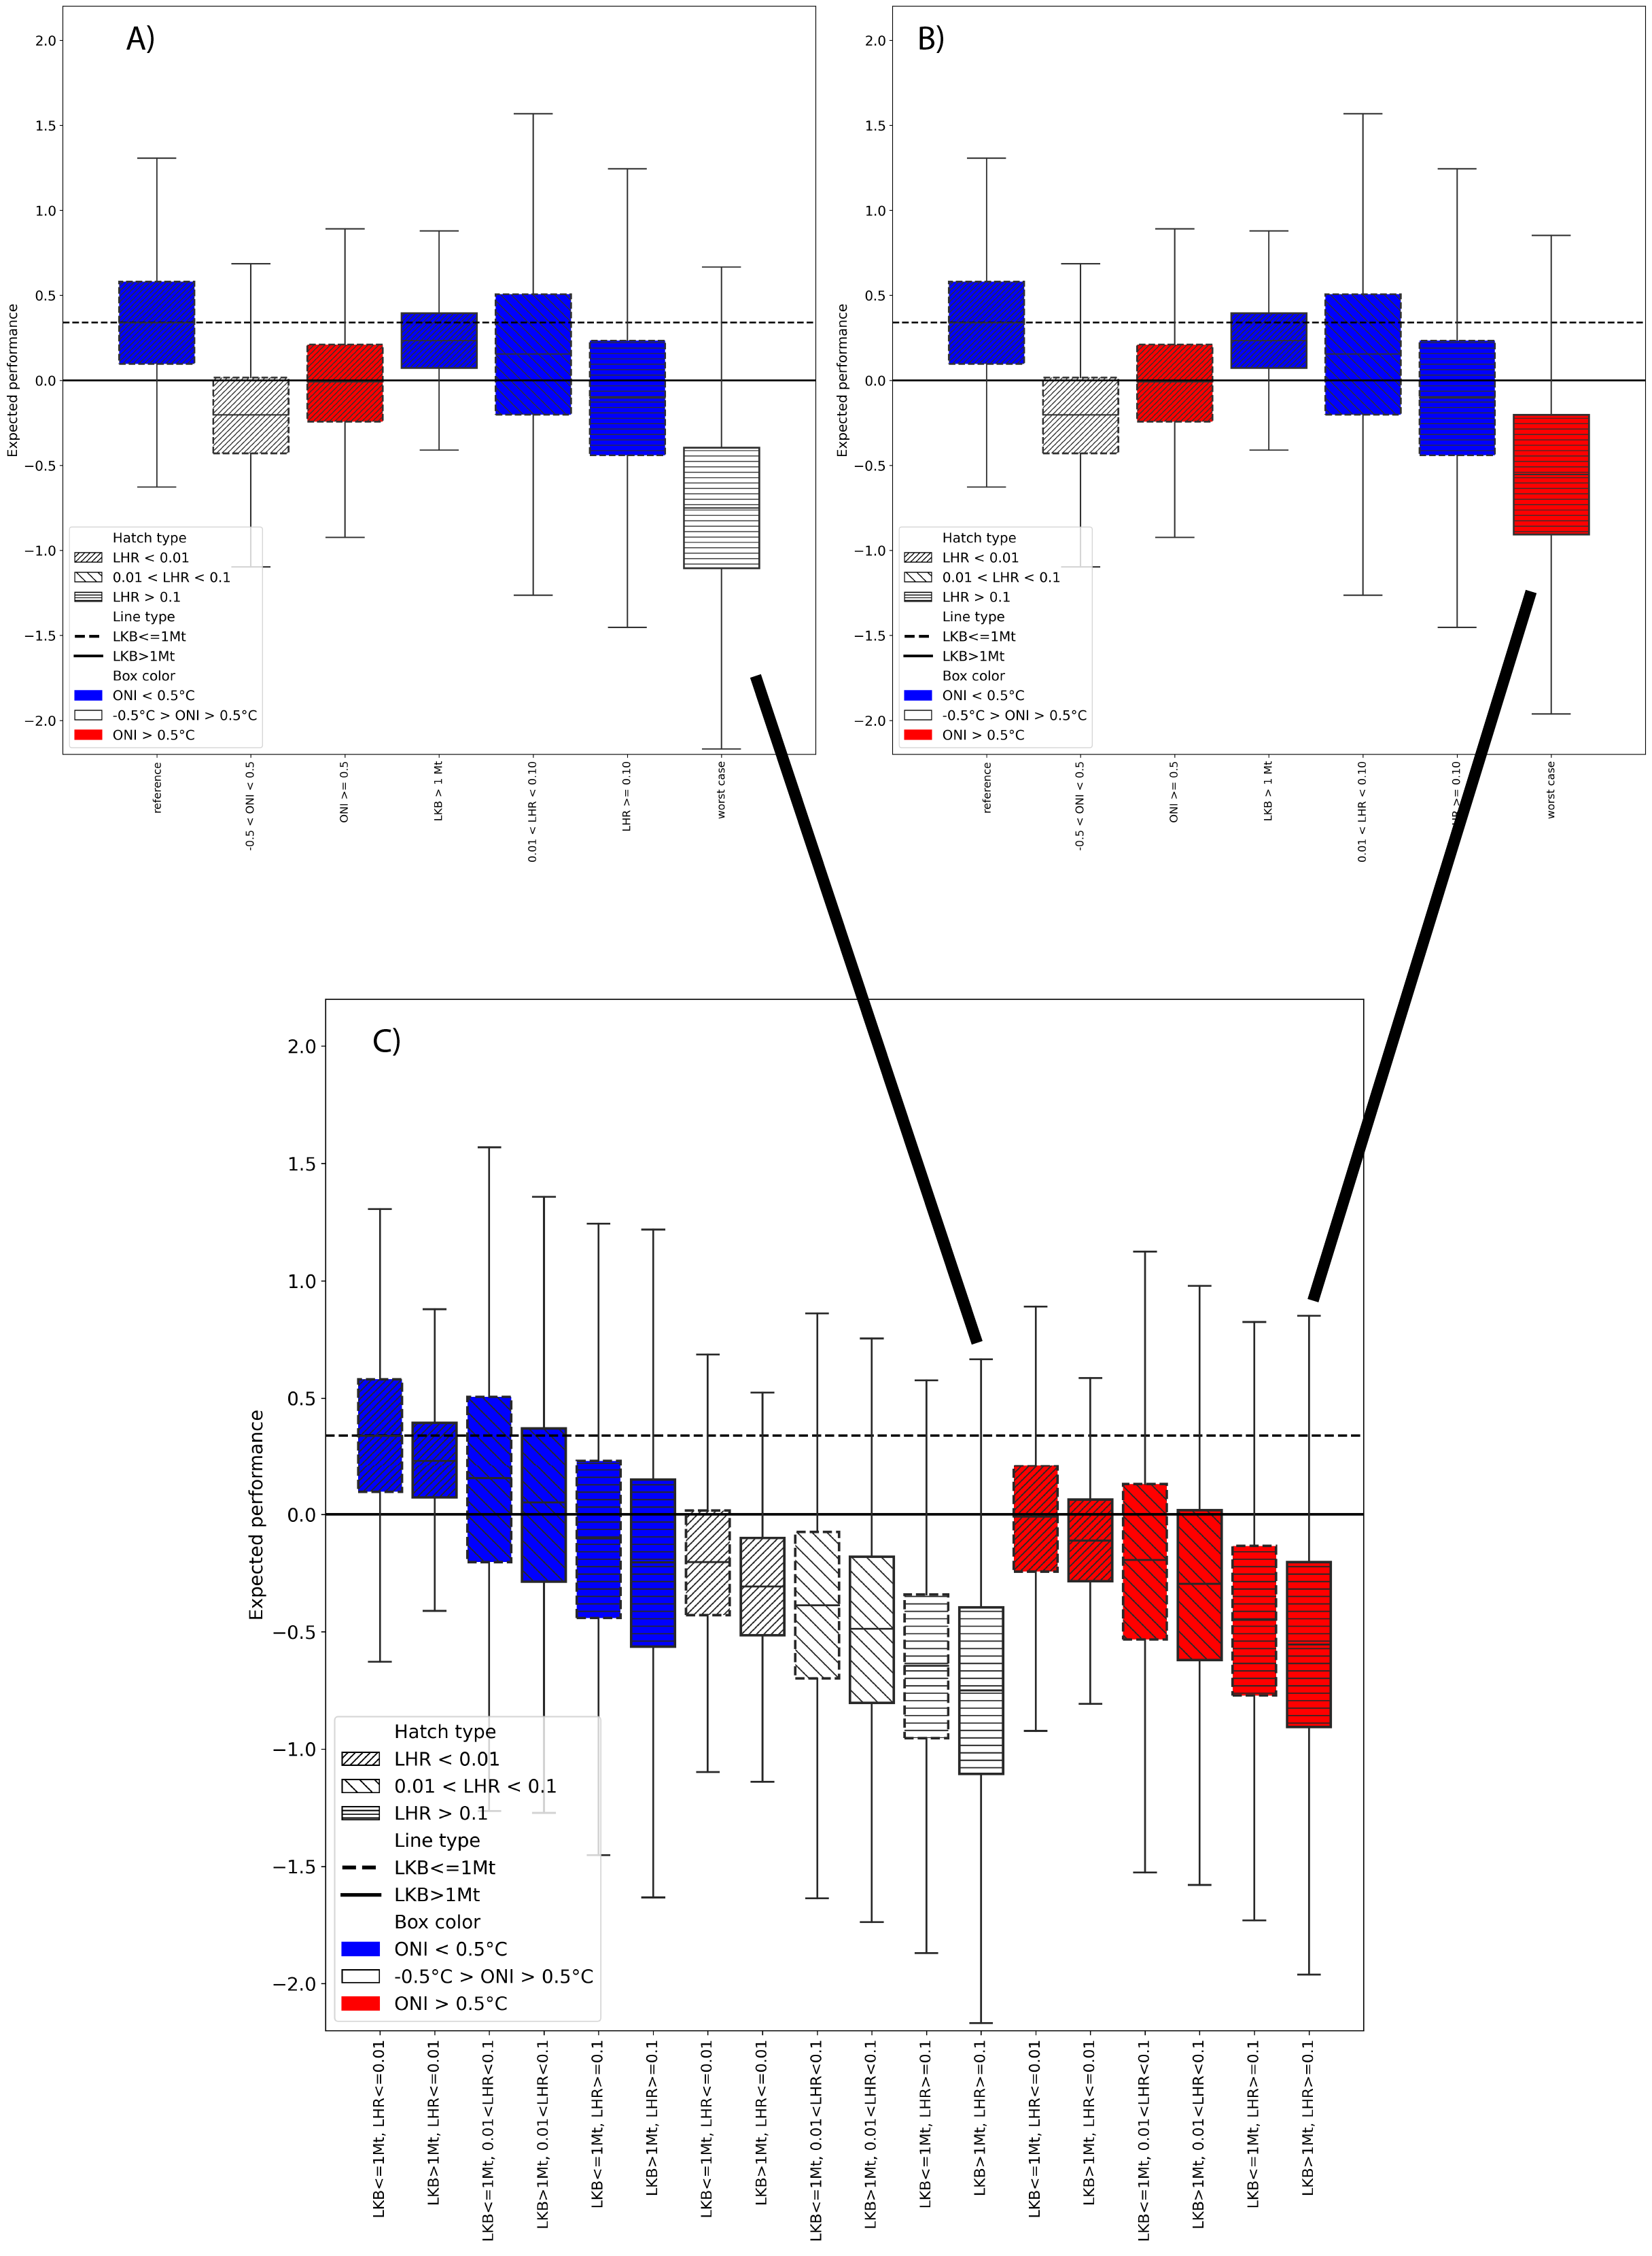
\includegraphics[width=0.75\linewidth]{./Watters EMM figures/Watters original and mistake} \caption{Original Figure 1 plot from Watters et al. 2020 with A) Neutral ONI and B) B) Warm ONI constituting the Worst Case selected.  C) Displays the original case-by-case plots recreated from the paper, with Case 12 representing the intention while data from Case 18 was selected for rendering the boxplot.  Note that the expected performance under neutral ONI Worst Case is poorer than under the warm ONI that was presented in the original paper.  Henceforth, to facilitate comparison, we refer to the ONI Neutral plot however we consider this unrealistic if the intention is to portray a Worst Case of a continuing warming climate.}\label{fig:Watters original and mistake}
\end{figure}

\begin{figure}

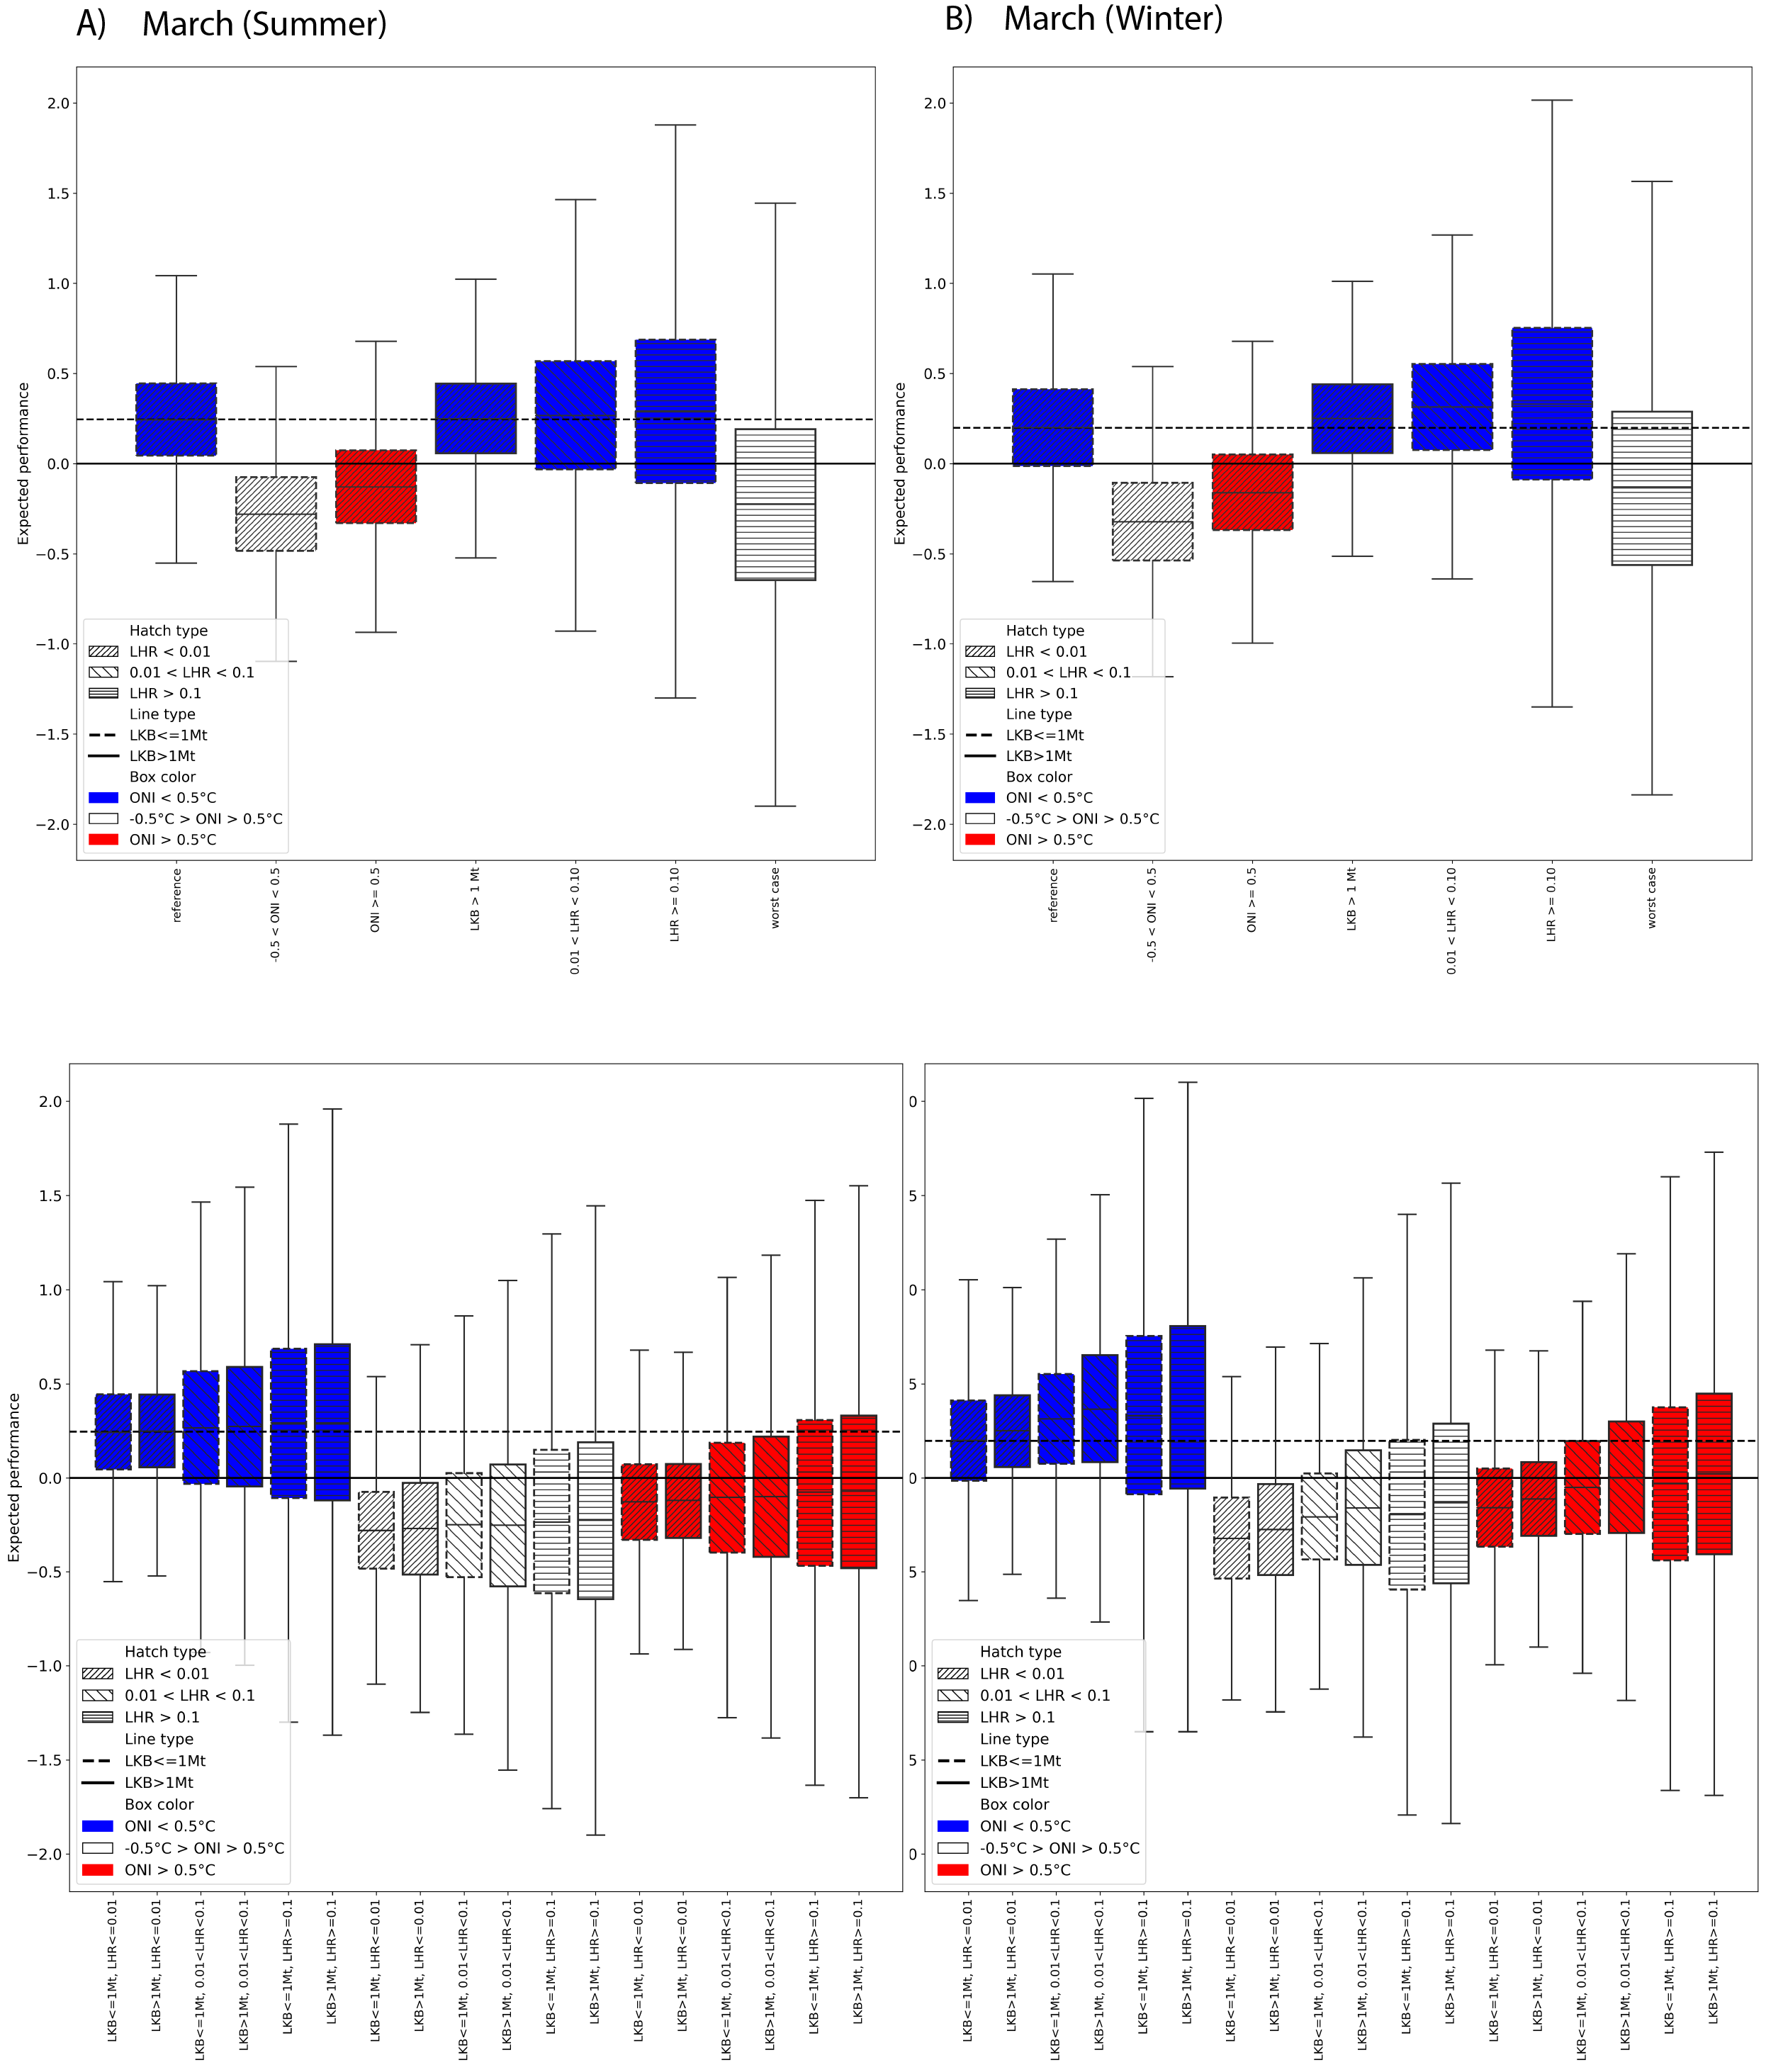
\includegraphics[width=1\linewidth]{./Watters EMM figures/All spp summer then winter 37} \hfill{}

\caption{Model output for the alternatve Watters et al. 2020 scenario outlined above (all species initially present, Adélie and chinstrap penguins migrate out of the area after breeding, LKB and LHR rescaled to SSMU and March included in summer or winter).   Selected cases as per Watters et al. 2020 for March in A) Summer and B) Winter are provided, with the corresponding case-by-case boxplots presented beneath.  Boxplots are colour-coded by ONI state (red=warm, white=neutral, blue=cold).  In all cases, the marginal effect of ONI dominated the expected performance of penguins against their long-term mean, irrespective of LKB or LHR.}\label{fig:Scenario plot 1}
\end{figure}

\begin{landscape}

\elandscape
\blandscape


\end{document}
